\documentclass[tikz,border=5pt]{standalone}
\usepackage{tikz}
\usetikzlibrary{arrows.meta,positioning}
\definecolor{nebula}{HTML}{6366F1}
\definecolor{spark}{HTML}{14B8A6}
\definecolor{ink}{HTML}{334155}
\begin{document}
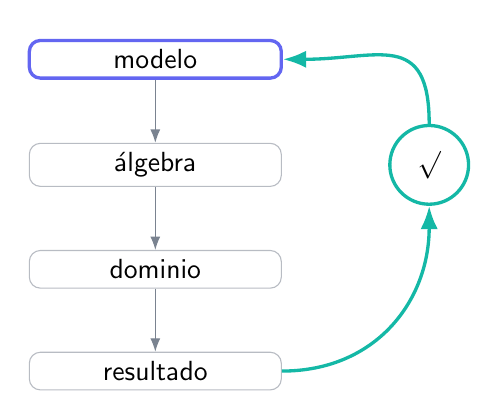
\begin{tikzpicture}[font=\sffamily,>=Latex,node distance=.8cm]
  \node[draw=nebula,very thick,rounded corners=4pt,minimum width=3.2cm] (m) {modelo};
  \node[draw=ink!35,rounded corners=4pt,below=of m,minimum width=3.2cm] (a) {álgebra};
  \node[draw=ink!35,rounded corners=4pt,below=of a,minimum width=3.2cm] (d) {dominio};
  \node[draw=ink!35,rounded corners=4pt,below=of d,minimum width=3.2cm] (r) {resultado};
  \node[draw=spark,very thick,circle,right=1.35cm of a,minimum size=1cm] (c) {$\surd$};
  \draw[->,ink!65] (m)--(a); \draw[->,ink!65] (a)--(d); \draw[->,ink!65] (d)--(r);
  \draw[->,very thick,spark] (r.east) .. controls +(1.2,0) and +(0,-1.2) .. (c.south);
  \draw[->,very thick,spark] (c.north) .. controls +(0,1.2) and +(1.2,0) .. (m.east);
\end{tikzpicture}
\end{document}
